%; whizzy chapter
% -initex iniptex -latex platex -format platex -bibtex jbibtex -fmt fmt
% 以上 whizzytex を使用する場合の設定。


%     Tokyo Debian Meeting resources
%     Copyright (C) 2009 Junichi Uekawa

%     This program is free software; you can redistribute it and/or modify
%     it under the terms of the GNU General Public License as published by
%     the Free Software Foundation; either version 2 of the License, or
%     (at your option) any later version.

%     This program is distributed in the hope that it will be useful,
%     but WITHOUT ANY WARRANTY; without even the implied warranty of
%     MERCHANTABILITY or FITNESS FOR A PARTICULAR PURPOSE.  See the
%     GNU General Public License for more details.

%     You should have received a copy of the GNU General Public License
%     along with this program; if not, write to the Free Software
%     Foundation, Inc., 51 Franklin St, Fifth Floor, Boston, MA  02110-1301 USA

%  preview (shell-command (concat "evince " (replace-regexp-in-string "tex$" "pdf"(buffer-file-name)) "&"))
% 画像ファイルを処理するためにはebbを利用してboundingboxを作成。
%(shell-command "cd image200903; ebb *.png")

%%ここからヘッダ開始。

\documentclass[mingoth,a4paper]{jsarticle}
\usepackage{monthlyreport}

% 日付を定義する、毎月変わります。
\newcommand{\debmtgyear}{2009}
\newcommand{\debmtgmonth}{3}
\newcommand{\debmtgdate}{21}
\newcommand{\debmtgnumber}{50}



\begin{document}

\begin{titlepage}
\thispagestyle{empty}

% タイトルページ:編集必要な部分は最初のマクロに飛ばすこと

\vspace*{-2cm}
第\debmtgnumber{}回 東京エリア Debian 勉強会資料

\hspace*{-2.4cm}
\includegraphics[width=210mm]{image200801/2008title.eps}\\
\hfill{}\debmtgyear{}年\debmtgmonth{}月\debmtgdate{}日

\end{titlepage}

\dancersection{Introduction}{上川 純一}

\begin{multicols}{2}
 
 
 今月のDebian勉強会へようこそ。これからDebianの世界にあしを踏み入れると
 いう方も、すでにどっぷりとつかっているという方も、月に一回Debianについ
 て語りませんか?

 Debian勉強会の目的は下記です。

 \begin{itemize}
 \item \underline{Debian Developer} (開発者)の育成。
 \item 日本語での「\underline{開発に関する情報}」を整理してまとめ、アップデートする。
 \item \underline{場}の提供。
 \begin{itemize}
  \item 普段ばらばらな場所にいる人々が face-to-face で出会える場を提供
	する。
  \item Debian のためになることを語る場を提供する。
  \item Debianについて語る場を提供する。
 \end{itemize}
 \end{itemize}		

 Debianの勉強会ということで究極的には参加者全員がDebian Packageをがりがり
 と作るスーパーハッカーになった姿を妄想しています。情報の共有・活用を通し
 て Debianの今後の能動的な展開への土台として、「場」としての空間を提供す
 るのが目的です。

 2009年の計画は仮です。

 \begin{enumerate}
  \item 新年の企画 (アンサンブル荻窪開催)
  \item OSC Tokyo
  \item VAIO P インストール記録、
	カーネル読書会 ディストリビューション大集合(小林さん)(東京大学?)
  \item Git Handson (岩松)(あんさんぶる荻窪?)
  \item 家Debianサーバ vs 職場のネットワーク(千代田区都立図書館?\footnote{\url{http://www.library.chiyoda.tokyo.jp/}})
  \item Asterisk (東京大学?)
  \item スペインにて開催
  \item Debconf報告会
  \item OSC Fall?
  \item udev + HAL(岩松さん)
  \item 3D graphics 開発(藤沢さん) 
  \item Debian サーバ+VMware + 各種OS、
	他の仮想化ツール(vserver etc.)、
	忘年会
 \end{enumerate}

 会場候補としては下記があります:

 \begin{itemize}
  \item 大学
  \item 恵比寿SGIホール
  \item Googleオフィス
  \item 公民館(あんさんぶる荻窪等)
  \item 都立会議室(無線LAN)
  \item 健保の施設
 \end{itemize}

\end{multicols}


\newpage

\begin{minipage}[b]{0.2\hsize}
 \definecolor{titleback}{gray}{0.9}
 \colorbox{titleback}{\rotatebox{90}{\fontsize{80}{80} {\gt デビアン勉強会} }}
\end{minipage}
\begin{minipage}[b]{0.8\hsize}
\hrule
\vspace{2mm}
\hrule
%
% there are too many entries in 200901, usually
% we have tocdepth=2.
%
\setcounter{tocdepth}{1}
\tableofcontents
\vspace{2mm}
\hrule
\end{minipage}

\dancersection{最近のDebian関連のミーティング報告}{上川 純一}
\subsection{東京エリアDebian勉強会48回目報告}
% (query-replace-regexp "<.*?>" "")
% (query-replace-regexp "^[	 ]\+" "")

2009年1月17日土曜日に
東京エリアDebian勉強会の
第48回
を開催しました。

今回の参加者は
id774さん、
あけどさん、
前田耕平さん、
小室文さん、
山本浩之さん、
岩松信洋さん、
やまだたくまさん、
じつかたさん、
キタハラさん、
小林儀匡さん、
藤沢理聡さん、
上川の12名でした。

クイズについては、今回は小林さんが当初不在だったのと
クイズを用意していなかったのでキャンセルです。
何か別の企画を期待したいところです。

最初に最近のイベントの紹介をしました。
前回の勉強会のおさらいと、
Debian JP で行ったIAX会議について紹介しました。
IAXでの音声会議に興味をそそられた人もいたようです。

\url{http://pspunch.com/pd/article/asterisk_meetme_ja.html}にて
今回利用した設定が紹介されています。

まず最初に事前課題を紹介しました。

2009年にどういう内容を実施するのかについて議論しました。
ブレインストーミングをしてそのあと2009年の毎月の計画をたてました。
今年は無事にできるかな?

最後に冬休みの宿題を発表しあって終了。

上川はGit format-patchを利用したワークフローでいかにコンフリクトを発生
させないかを紹介しました。
前田さんはMacBookにLennyをインストールしなおしたときにはまった内容。
小室さんは、Google Ajax API の紹介。
id774さんはAspire One にインストールしたときの話。
山本浩之さんは2chビューアーパッケージについて。
岩松さんは Linux Kernel の .config 自動生成ツールについての紹介でした。

\subsection{東京エリアDebian勉強会49回目報告}
% (query-replace-regexp "<.*?>" "")
% (query-replace-regexp "^[	 ]\+" "")

第49回東京エリアDebian勉強会はOSC2009 Tokyo/Spring@日本電子専門学校に参加してきました。

セミナーとしてはハンズオンを二枠行い、CDBSを用いたDebianパッケージ作成を伝授しました。
参加者は全員で30名強、当日飛び入りが4名いました。
ハンズオンをやってみると、参加者のスキルレベルが予想以上にまちまちで、慣れない人だとスペルミスだけでもつまづいてしまい、前準備だけでも30分程かかってしまうことなどが分かって来ました。
時間内に最後まで課題を終えられた人は半分ぐらいでした。終わらなかった残りの人には、宿題としておきました。
しかし、ほとんどの人が時間内に課題をクリアできなかった、昨年のハンズオンよりは一歩前進です。

ブースではDebian on ChumbyやDebian on EeePCの展示や、リリースされたばかりのLennyで作ったLive DVDの配布などを行いました。
会場の都合でブースのスペースがとても狭く、初めての人には近寄り難かったかもしれませんが、それでも用意していたDVD、40枚程がほぼ無くなってしまうほど好評でした。

%\subsection{Ubuntu XXX}
%
%TODO: やまねさんが書く?
%
%\subsection{Linux Consortium 10 years event }
%
%TODO: 
%\url{http://www.debian.or.jp/blog/events/linuxconsortium10th.html}
%についてやまねさんが書く?

%============================================================
%%% trivia quiz
\dancersection{Debian Trivia Quiz}{岩松 信洋}

ところで、みなさん Debian 関連の話題においついていますか?Debian関連の話
題はメーリングリストをよんでいると追跡できます。ただよんでいるだけではは
りあいがないので、理解度のテストをします。特に一人だけでは意味がわからな
いところもあるかも知れません。みんなで一緒に読んでみましょう。

今回の出題範囲は\url{debian-devel-announce@lists.debian.org} に投稿された
内容とDebian Project Newsからです。

\begin{multicols}{2}
 %; whizzy-master ../debianmeetingresume200903.tex
% 以上の設定をしているため、このファイルで M-x whizzytex すると、whizzytexが利用できます。

 \santaku
 {2月14日にリリースされたのは}
 {etch}
 {sarge}
 {lenny}
 {C}
{}

 \santaku
 {3月12日にリリースされた Debian Policy のバージョンは}
 {3.8.0}
 {3.8.1}
 {3.8.2}
 {B}
{}

 \santaku
 {Debian Data Export は何か}
 {Debianパッケージに関するデータを容易に取り寄せるためのインターフェイス}
 {全世界にある、あらゆるデータをDebianパッケージ化するプロジェクト}
 {DebianのあらゆるデータをGoogleにすべて喰わせてみましたというプロジェクト}
 {A}
{}

 \santaku
 {Olivier BergerがMLに流したbts-linkに関する情報は}
 {bts-linkのソース管理リポジトリが壊れました}
 {bts-linkでリンクできるBTSを増やしました}
 {bts-linkサービスは終了です}
 {B}
{}

 \santaku
 {Debian FTP masterが変わりました。誰が新しく入ったでしょうか。}
 {Kei Hibino}
 {Ryan Murray}% FTP master を辞めた人
 {Mark Hymers}% 新しく入った人
 {C}
{}

 \santaku
 {3月16日にJoerg JaspertがMLに流したアナウンスは}
 {Debian の新しいロゴが決まりました}
 {パッケージのセクションが追加されます}
 {いくつかのディストリビューションと吸収合併します}
 {B}
{}

 \santaku
 {3月21日にリリースされた pbuilder のバージョンは?}
 {0.187}
 {1.298}
 {3.1}
 {A}
{}

 \santaku
 {Debian.org DPL に立候補していないのは}
 {Stefano Zacchiroli}
 {Steve McIntyre}
 {Nobuhiro Iwamatsu}
 {C}
{}

 \santaku
 {Debian JP 選挙の立候補しめきりは?}
 {3月20日}
 {3月22日}
 {3月24日}
 {B}
{}

\end{multicols}


% ===============================================================
\dancersection{研究室のソフトウェアを Debian パッケージにしてみる}{藤澤 徹}
\index{debhelper}
\index{gxp}
\index{mcmpi}
% ===============================================================

\subsection{対象とするソフトウェア}

今回パッケージにしてみるソフトウェアは東京大学 近山・田浦研究室で開発されている
グリッド用の MPI ライブラリである MC-MPI,
および MC-MPI を動作させるのに必要となる,
同じく近山・田浦研究室で開発されている並列分散シェルの GXP の 2 つです.

\subsection{パッケージにするに際して}

ソフトウェアをパッケージにするには, そのソフトウェアの構成と特徴をよく
理解する必要があります.以下にそれぞれのソフトウェアの特徴のうち,
パッケージを作る際に関係のありそうな事を並べます.

\subsubsection{MC-MPI}

MC-MPI は主に C 言語で記述されたコンパイラとライブラリによって構成されています.
また, 一部に Fortran のコードも含まれており, Fortran インターフェースも
持っていますが, これはオブションによりオフにする事もできます.

Autotools を使用しており, \verb|./configure && make && make install| という
見慣れたコマンドによってビルド, インストールする事ができます.

\subsubsection{GXP}

GXP は Python で記述されたコマンドと,
そのコマンドが必要とする Python モジュールによって構成されています.

インストールする, という作業は想定されておらず,
ダウンロードして展開して出てきたディレクトリをどこかに置き,
そこにパスを通して使うように作られています.

\subsection{使用するツール}

Debian のパッケージを作成する方法にはいくつかあるらしいのですが,
今回は debhelper を使用してみます.

\subsection{とりあえず動かしてみる}

とりあえずは自分の環境で動く事を確かめるため, パッケージとは関係なく
使ってみます.

MC-MPI は GXP を必要とするので, まず GXP から試してみましょう.

\subsubsection{GXP を使ってみる}

以下のサイトから執筆時点で最新版である \verb|gxp-3.05.tar.bz2| をダウンロードし, 展開します.

\begin{center}
\url{http://www.logos.t.u-tokyo.ac.jp/gxp/}
\end{center}

\begin{commandline}
$ mkdir gxp
$ cd gxp
$ # なんとかして gxp-3.05.tar.bz2 を持ってくる
$ tar jxvf gxp-3.05.tar.bz2
$ cd gxp-3.05
\end{commandline}

さて, GXP はインストール不要なので, このままでも動きます.
GXP の制御は全て \verb|gxpc| コマンドで行います.

\begin{commandline}
$ ./gxpc
gxpc: no daemon found, create one
/tmp/gxp-***-default/gxpsession-***-***-2009-03-20-06-46-07-15360-92311801
\end{commandline}

問題なく動いているようです.

\subsubsection{MC-MPI を使ってみる}

以下のサイトから執筆時点で最新版である \verb|mcmpi-0.21.0.tar.gz| をダウンロードし, 展開します.

\begin{center}
\url{http://www.logos.ic.i.u-tokyo.ac.jp/~h_saito/mcmpi/}
\end{center}

\begin{commandline}
$ mkdir mcmpi
$ cd mcmpi
$ # なんとかして mcmpi-0.21.0.tar.gz を持ってくる
$ tar zxvf mcmpi-0.21.0.tar.gz
$ cd mcmpi-0.21.0
\end{commandline}

前述のとおり, Autotools を使用しているので以下の見慣れたコマンドを打ちます.

\begin{commandline}
$ ./configure
$ make
$ sudo make install
\end{commandline}

サンプルプログラムが付属しているので,
これを \verb|mpicxx| でコンパイルしてみます.

\begin{commandline}
$ cd app
$ mpicxx -o hello ./hello.cpp
printf: 28: %q: invalid directive
printf: 28: %q: invalid directive
printf: 28: %q: invalid directive
[ g++ -I/usr/local/include    /usr/local/lib/libmpigxp.a -lresolv -lpthread -lnsl -lm  ]
/usr/lib/gcc/i486-linux-gnu/4.3.2/../../../../lib/crt1.o: In function `_start':
(.text+0x18): undefined reference to `main'
collect2: ld はステータス 1 で終了しました
\end{commandline}

おや, 動かないようです.
調べてみたところどうやら \verb|%q| は使えない事もあるようです.
これは文字列を必要ならばクォートするという指定子なので (おそらく),
サクッと \verb|\"%s\"| に置き換えてしまいます.
\verb|util| 以下の \verb|mpicc.in|, \verb|mpicxx.in|, \verb|mpif77.in| に修正を加え, ビルドし直します.

\begin{commandline}
$ cd ..
$ make distclean
$ ./configure
$ make
$ sudo make install
\end{commandline}

さて改めてコンパイルします.

\begin{commandline}
$ cd app
$ mpicxx -o hello ./hello.cpp
[ g++ -I/usr/local/include "-o" "hello" "./hello.cpp" /usr/local/lib/libmpigxp.a -lresolv -lpthread -lnsl -lm  ]
\end{commandline}

今度は上手くいったようです.
では実行してみましょう.
まず GXP で \verb|localhost| のみのクラスタを指定し, カレントディレクトリに移動します.
そこで \verb|mpirun| によって実行を開始します.

\begin{commandline}
$ gxpc
$ gxpc use ssh localhost
$ gxpc explore localhost
$ gxpc cd `pwd`
$ mpirun -np 1 ./hello
/usr/local/bin/mpirun: 157: Bad substitution
\end{commandline}

おや, またしても失敗です.
該当行を見ても

\begin{commandline}
done
\end{commandline}

と, よく分からない感じですが, よく調べてみると

\begin{commandline}
        if [ "$CONF_OPT" == "" -o "${CONF_OPT:0:1}" == "#" ] ; then
\end{commandline}

の行で落ちています.

\verb|${CONF_OPT:0:1}| という書き方は Bash では動きますが POSIX Shell では
動かないようなので, とりあえず Bash で動かすように変更してしまいます.

\begin{commandline}
$ cd ..
$ make distclean
$ ./configure
$ make
$ sudo make install
\end{commandline}

では改めて実行しましょう.

\begin{commandline}
$ cd app
$ mpirun -np 1 ./hello
INFO: _exchange_end_points: 42498
INFO: _measure_latencies: 23884
INFO: _create_bounding_graph: 26520
INFO: _create_routing_table: 57663
INFO: _create_spanning_tree: 20144
INFO: Env_Init: 172304
Hello 0/1
\end{commandline}

今度こそ見事動きました.

\subsection{MC-MPI のパッケージ作成}

まずは MC-MPI のパッケージを作成します.

\subsubsection{準備}

とりあえずさっきとは別のディレクトリで作業をしたほうが良さそうです.

\begin{commandline}
$ mkdir deb_mcmpi
$ cd deb_mcmpi
$ # なんとかして mcmpi-0.21.0.tar.gz を持ってくる
$ tar zxvf mcmpi-0.21.0.tar.gz
$ cd mcmpi-0.21.0
\end{commandline}

ここでさっきのバグの修正を加えておきます.

\subsubsection{さらに修正}

MC-MPI では自身のバージョンを \verb|/usr/etc/VERSION| に記述する事になっているのですが,
これはビミョーなので \verb|/usr/share/mcmpi/VERSION| あたりに変更しておきます.
変更するファイルは以下のとおりです.

\begin{itemize}
 \item \verb|etc/Makefile.in|
 \item \verb|util/mpicc.in|
 \item \verb|util/mpicxx.in|
 \item \verb|util/mpif77.in|
 \item \verb|util/mpirun.in|
\end{itemize}

\subsubsection{パッケージ情報記述用のファイルの作成}

パッケージを作成する場合にはソフトウェア本体はもちろんの事,
インストール方法や依存関係等, そのパッケージの情報を記述したファイルが
必要になります.

\verb|dh_make| コマンドを使用するとこれらを記述するためのファイルの雛形を
作成してくれます.
この際, \verb|DEBFULLNAME|, \verb|DEBEMAIL| 変数により作者情報を指定できます.
この名前, メールアドレスが GPG の鍵の情報と一致しないと
作成したパッケージにサインできないので困ります.

\begin{commandline}
$ export DEBFULLNAME="Tooru Fujisawa"
$ export DEBEMAIL="arai_a@mac.com"
$ dh_make -e arai_a@mac.com -f ../mcmpi-0.21.0.tar.gz
Type of package: single binary, multiple binary, library, kernel module or cdbs?
 [s/m/l/k/b]
> s

Maintainer name : Tooru Fujisawa
Email-Address   : arai_a@mac.com 
Date            : Fri, 20 Mar 2009 06:55:00 +0900
Package Name    : mcmpi
Version         : 0.21.0
License         : blank
Using dpatch    : no
Type of Package : Multi-Binary
Hit <enter> to confirm: 
> [ENTER]
\end{commandline}

途中で \verb|Type of package| と聞かれます.
MC-MPI はライブラリも含みますが, メインはコンパイラ等なので
とりあえず \verb|single binary| を選んでおけばよさそうです.

\subsubsection{パッケージ情報記述用のファイルの修正}

さて, さきほどの \verb|dh_make| によって, \verb|debian| というディレクトリが作成され,
この中にいろいろなファイルが並んでいます.

この中で重要なのは次のものです.

\begin{itemize}
 \item \verb|changelog|
 \item \verb|copyright|
 \item \verb|dirs|
 \item \verb|control|
 \item \verb|rule|
\end{itemize}

順番に修正していきましょう.

\subsubsubsection{changelog}

これはパッケージの更新履歴です.
ソフトウェア本体の更新履歴とは別モノです.
とりあえず雛形に沿って以下のようにしておきます.

\begin{commandline}
mcmpi (0.21.0-1) unstable; urgency=low

  * Initial release

 -- Tooru Fujisawa <arai_a@mac.com>  Fri, 20 Mar 2009 06:55:00 +0900
\end{commandline}

\subsubsubsection{copyright}

これはソフトウェアの著作権情報を記述するファイルです.
雛形に沿ってダウンロード元, 元々の作者, ライセンス等を記述します.

\begin{commandline}
This package was debianized by Tooru Fujisawa <arai_a@mac.com> on
Fri, 20 Mar 2009 06:55:00 +0900.

It was downloaded from http://www.logos.ic.i.u-tokyo.ac.jp/~h_saito/mcmpi/

Upstream Author(s):
    Hideo Saito <h_saito@logos.ic.i.u-tokyo.ac.jp>

Copyright:
    (c) 2007 Hideo Saito. All Rights Reserved.

License:
    GPL Version 2

The Debian packaging is (C) 2009, Tooru Fujisawa <arai_a@mac.com> and
is licensed under the GPL, see `/usr/share/common-licenses/GPL'.
\end{commandline}

\subsubsubsection{dirs}

これはパッケージ作成時に自動的に作成してほしいディレクトリを
記述するファイルです.
デフォルトでは \verb|usr/bin| と \verb|usr/sbin| が入っていますが,
\verb|usr/sbin| は要らないので削除してしまいます.
また, \verb|VERSION| を \verb|usr/share/mcmpi| にコピーするようにしたので
これを追加します.

\begin{commandline}
usr/bin
usr/share/mcmpi
\end{commandline}

\subsubsubsection{control}

これはパッケージの依存関係や説明を記述するファイルです.

雛形通りに進むと, まず \verb|Homepage| にダウンロード元を書き,
\verb|Depends| に次に作成する \verb|gxp| を追加しておきます.
また, バグ修正の際に Bash を使用する事にしたので \verb|bash| も追加します.
最後に説明を短いものと長いものと書いておきます.

\begin{commandline}
Source: mcmpi
Subsection: unknown
Priority: extra
Maintainer: Tooru Fujisawa <arai_a@mac.com>
Build-Depends: debhelper (>= 7), autotools-dev
Standards-Version: 3.7.3
Homepage: http://www.logos.ic.i.u-tokyo.ac.jp/~h_saito/mcmpi/

Package: mcmpi
Architecture: any
Depends: ${shlibs:Depends}, ${misc:Depends} bash gxp
Description: Grid-enabled implementation of MPI
  MC-MPI is a Grid-enabled implementation of MPI, developed by Hideo
  Saito at the University of Tokyo.  Its main features include the
  following:
  - [Firewall and NAT traversal]: MC-MPI constructs an overlay
    network, allowing nodes behind firewalls and nodes without global
    IP addresses to participate in computations.  There is no need to
    perform maual configuration; MC-MPI automatically probes
    connectivity, selects which connections to establish, and performs
    routing.
  - [Locality-aware connection management]: Establishing too many
    connections, especially wide-area connections, results in many
    problems, including but not limited to the follwing: exhaustion of
    system resources (e.g., file descriptors, memory), high message
    reception overhead, and congestion between clusters during
    all-to-all communication.  Therefore, MC-MPI limits the number of
    connections that are established.  If we assume, for simplicity,
    that n processes are distributed equally among c clusters, then at
    most O(log n) connections are established by each process and at
    most O(n log c) connections are established between clusters.  As
    MC-MPI uses a lazy connect strategy, fewer connections are
    established for applications in which few process pairs
    communicate.  The maximum number of connections allowed can be
    controlled by passing the -beta option to mpirun (see Subsection 3).
  - [Locality-aware rank assignment]: Temporarily disabled in this
    version.
\end{commandline}

\subsubsubsection{rule}

これはビルドやパッケージの方法を記述する \verb|Makefile| です.
MC-MPI の場合には Autotools を使っているので得に変える所は無いハズです.
(実はありますがそれは後述...)

\subsubsection{ソースパッケージの作成}

準備が出来たら \verb|debuild| コマンドでパッケージを作成します.
ソースパッケージとバイナリパッケージの両方を作ってみます.

まずはソースパッケージです.

\begin{commandline}
$ debuild -S
\end{commandline}

小人さんが頑張ってくれた後, サインをするためのパスフレーズを聞いてくるので
2 回くらい入力します.

するとソースパッケージの完成です.
上のディレクトリに色々出来ています.

\subsubsection{バイナリパッケージの作成}

さて, 続いてバイナリパッケージです.

\begin{commandline}
$ debuild
\end{commandline}

\verb|configure|, \verb|make| なんかが走っている様子が流れていきます.

\begin{commandline}
fortran/.libs/libfortran.a(farg.o): In function `mpigxp_getarg':
*/deb_mcmpi/mcmpi-0.21.0/src/fortran/farg.f:9: undefined reference to `_gfortran_getarg_i4'
fortran/.libs/libfortran.a(farg.o): In function `mpigxp_iargc':
*/deb_mcmpi/mcmpi-0.21.0/src/fortran/farg.f:2: undefined  reference to `_gfortran_iargc'
fortran/.libs/libfortran.a(initf.o): In function `mpi_init__':
*/deb_mcmpi/mcmpi-0.21.0/src/fortran/initf.c:16: undefined reference to `mpigxp_iargc__'
*/deb_mcmpi/mcmpi-0.21.0/src/fortran/initf.c:20: undefined reference to `mpigxp_getarg__'
collect2: ld returned 1 exit status
\end{commandline}

超怒られました. しかも私の知らない Fortran のコードです.
調べてみたところ, この関数は処理系によっては勝手に作られるものだそうで,
gFortran は作らないようです.
解決する方法が分からないので, ここはいさぎよく Fortran インターフェースを
無効にして作り直しましょう.

\verb|debian/rule| ファイルの中で, \verb|./configure| してる行に \verb|--disable-f77| を追加します

\begin{commandline}
        ./configure $(CROSS) --prefix=/usr --mandir=\$${prefix}/share/man --infodir=\$${prefix}/share/info \
        CFLAGS="$(CFLAGS)" LDFLAGS="-Wl,-z,defs" --disable-f77
\end{commandline}

改めてビルドします.

\begin{commandline}
$ debuild
...
/usr/bin/install -c -d /usr/etc
/usr/bin/install: `/usr/etc' の属性を変更できません: No such file or directory
\end{commandline}

またまた怒られました.
debuild は \verb|debian/mcmpi/| 以下にソフトウェアをインストールして
パッケージにするハズなのに, 外にインストールしようとしています.
これは \verb|rule| ファイルからディレクトリを \verb|DESTDIR| として
渡しているのに, \verb|Makefile| の方が対応していないためです.

\verb|etc/Makefile.in|, \verb|util/Makefile.in|, の中で \verb|prefix| に
\verb|DESTDIR| を追加します.

\begin{commandline}
prefix = $(DESTDIR)@prefix@
\end{commandline}

\begin{commandline}
$ debuild
\end{commandline}

今度は成功しました.

上のディレクトリに \verb|mcmpi_0.21.0-1_i386.deb| が出来ています.

\subsubsection{インストールテスト}

依存関係が正しいかどうか, インストールしてみましょう.

\begin{commandline}
$ cd ..
$ sudo dpkg -i mcmpi_0.21.0-1_i386.deb
未選択パッケージ mcmpi を選択しています。
(データベースを読み込んでいます ... 現在 219582 個のファイルとディレクトリがインストールされています。)
(mcmpi_0.21.0-1_i386.deb から) mcmpi を展開しています...
dpkg: 依存関係の問題により mcmpi の設定ができません:
 mcmpi は以下に依存 (depends) します: gxp ...しかし:
  パッケージ gxp はまだインストールされていません。
dpkg: mcmpi の処理中にエラーが発生しました (--install):
 依存関係の問題 - 設定を見送ります
以下のパッケージの処理中にエラーが発生しました:
 mcmpi
\end{commandline}

\verb|gxp| が無いと言われました. 予定通り作成できているようです.
とりあえず削除しておきます.

\begin{commandline}
$ sudo apt-get remove --purge mcmpi
\end{commandline}

\subsection{GXP のパッケージ作成}

さて, 無いと言われた GXP パッケージの方を作ります.

\subsubsection{準備}

こちらもさっきとは別のディレクトリで作業をします.
ただし今回, 作業を開始した時点では 3.03 が最新バージョンだったので,
バージョンアップのテストも兼ねて 3.03 のパッケージをまず作ります.

\begin{commandline}
$ mkdir deb_gxp
$ cd deb_gxp
$ # なんとかして gxp-3.03.tar.bz2 を持ってくる
$ tar jxvf gxp-3.03.tar.bz2
$ cd gxp-3.03
\end{commandline}

\subsubsection{パッケージ情報記述用のファイルの作成}

ほぼ同様です.

\begin{commandline}
$ export DEBFULLNAME="Tooru Fujisawa"
$ export DEBEMAIL="arai_a@mac.com"
$ dh_make -e arai_a@mac.com -f ../gxp-3.03.tar.bz2 
Type of package: single binary, multiple binary, library, kernel module or cdbs?
 [s/m/l/k/b]
> s

Maintainer name : Tooru Fujisawa
Email-Address   : arai_a@mac.com 
Date            : Fri, 20 Mar 2009 07:15:35 +0900
Package Name    : gxp
Version         : 3.03
License         : blank
Using dpatch    : no
Type of Package : Single
Hit <enter> to confirm: 
> [ENTER]
\end{commandline}

GXP は外から見ればコマンド 1 つなので, これも \verb|single binary| で
よさそうです.

\subsubsection{パッケージ情報記述用のファイルの修正}

さて, これらを記述する前に考えなければならない事があります.
GXP はインストールを想定されていないため, パッケージにした場合に
どこに置いてどのように使うかを決めなければいけません.

今回は \verb|/usr/share/gxp| 以下にファイルをコピーし,
\verb|/usr/bin/gxpc| を \verb|/usr/share/gxp/gxpc| にリンクする事にします.

\subsubsubsection{changelog}

特に変わった事はしません.

\begin{commandline}
gxp (3.03-1) unstable; urgency=low

  * Initial release

 -- Tooru Fujisawa <arai_a@mac.com>  Fri, 20 Mar 2009 07:15:35 +0900
\end{commandline}

\subsubsubsection{copyright}

こちらも特に変わった事はしません.

\begin{commandline}
This package was debianized by Tooru Fujisawa <arai_a@mac.com> on
Fri, 20 Mar 2009 07:15:35 +0900.

It was downloaded from http://www.logos.t.u-tokyo.ac.jp/gxp/

Upstream Author(s): 
    Dun Nan
    Kenjiro Taura 
    Yoshikazu Kamoshida 

Copyright:
    (c) 2008 by Kenjiro Taura. All rights reserved.
    (c) 2007 by Kenjiro Taura. All rights reserved.
    (c) 2006 by Kenjiro Taura. All rights reserved.
    (c) 2005 by Kenjiro Taura. All rights reserved.

License:
    GPL Version 2

The Debian packaging is (C) 2009, Tooru Fujisawa <arai_a@mac.com> and
is licensed under the GPL, see `/usr/share/common-licenses/GPL'.
\end{commandline}

\subsubsubsection{dirs}

さて, GXP はインストーラを持っていないので,
インストールのコードは直接 \verb|rule| に書く事になります.
できるだけ作業を減らしたいので, 必要なディレクトリはこちらに全部書いてしまいましょう.

\begin{commandline}
usr/bin
usr/share
usr/share/gxp
\end{commandline}

\subsubsubsection{control}

GXP は Python のモジュールを内部に持っているので,
これらをインストール先でバイトコードにコンパイルしてあげる作業を
してあげなければいけません.
この作業を勝手にしてくれるのが \verb|dh_pycentral| です.
このために, 2 箇所に \verb|XS-Python-Version: all| を追加します.

また, GXP は環境にアーキテクチャに依存しないので, \verb|Architecture| を
\verb|all| にします.
ただし, 実行に Python が必要になるので \verb|Depends| に \verb|python| を,
また前述の作業のために \verb|dh_pycentral| が必要になるので,
\verb|Depends|, \verb|Build-Depends| に \verb|python-central| を追加します.

\begin{commandline}
Source: gxp
Subsection: unknown
Priority: extra
Maintainer: Tooru Fujisawa <arai_a@mac.com>
Build-Depends: debhelper (>= 7)
Standards-Version: 3.7.3
XS-Python-Version: all
Homepage: http://www.logos.t.u-tokyo.ac.jp/gxp/

Package: gxp
Architecture: all
Depends: ${shlibs:Depends}, ${misc:Depends}, python
XS-Python-Version: all
Description: parallel/distributed shell
 GXP is a parallel/distributed shell, plus a parallel task execution engine
 that runs your Makefile in parallel on distributed machines.
 Very easy to install
 (no need to compile. install it on YOUR machine and use it on ALL machines). 
\end{commandline}

\subsubsubsection{rule}

まず, \verb|Makefile| が無いので \verb|$(MAKE)| と入った行は全てコメントアウトします.

そして, \verb|$(MAKE) DESTDIR=$(CURDIR)/debian/gxp install| の行の後に
次のようなインストールのコマンドを追加します.
展開して出てきたもの全部, としたいのですが, \verb|debian| ディレクトリがあるので
ファイルを並べます.

\begin{commandline}
        cp -r ChangeLog License README doc ex expectd.py gxpbin gxpc gxpc.py gxpd.py gxpm.py ifconfig.py inst_local.py \
        inst_remote.py inst_remote_stub.py ioman.py misc mkrelease opt.py $(CURDIR)/debian/gxp/usr/share/gxp
        ln -s $(CURDIR)/debian/gxp/usr/share/gxp/gxpc $(CURDIR)/debian/gxp/usr/bin/gxpc
\end{commandline}

また, \verb|dh_pycentral| を動かすために, \verb|dh_python| の次の行あたりに
\verb|dh_pycentral| と書いておきます.

\begin{commandline}
#       dh_python
        dh_pycentral
\end{commandline}

\subsubsection{ソースパッケージの作成}

まずはソースパッケージを作ります.

\begin{commandline}
$ debuild -S
\end{commandline}

何事もなく完了します.

\subsubsection{バイナリパッケージの作成}

さて, 続いてバイナリパッケージです.

\begin{commandline}
$ debuild
...
E: gxp: missing-dep-for-interpreter expect => expect (./usr/share/gxp/gxpbin/ssh_passwd)
E: gxp: missing-dep-for-interpreter expect => expect (./usr/share/gxp/gxpbin/su_cmd)
...
\end{commandline}

途中でエラーが出ています.
これは \verb|ssh_passwd|, \verb|su_cmd| が \verb|/usr/bin/expect| を使用しているのに,
\verb|Depends| に入っていないという事なので, \verb|debian/control| を更新します.

\begin{commandline}
Depends: ${shlibs:Depends}, ${misc:Depends}, python, python-central, expect
\end{commandline}

ではビルドし直します.

\begin{commandline}
$ debuild
\end{commandline}

今度は何事もなく完了し, 上のディレクトリに \verb|gxp_3.03-1_all.deb| が
できています.

\subsubsection{バージョンアップ}

さて, 作業をしている間に GXP の新しいバージョン 3.05 がリリースされたので
これをパッケージに反映します.

debhelper には新しいバージョンのチェック, 更新を自動化するための機構があります.
\verb|debian/watch| ファイルに以下のように記述します.
(というか, SourceForge なモノは例にあるので拡張子だけ変えます)

\begin{commandline}
version=3
http://sf.net/gxp/gxp-(.*)\.tar\.bz2
\end{commandline}

2行目が最新バージョンの URL のパターンです.
ここから自動的に最新バージョンを探して落としてくれます.

\begin{commandline}
$ uscan -verbose
-- Scanning for watchfiles in .
-- Found watchfile in ./debian
-- In debian/watch, processing watchfile line:
   http://sf.net/gxp/gxp-(.*)\.tar\.bz2
-- Found the following matching hrefs:
     /sites/download.sourceforge.net/pub/sourceforge/g/gx/gxp/gxp-3.02.tar.bz2
     /sites/download.sourceforge.net/pub/sourceforge/g/gx/gxp/gxp-3.02.tar.bz2
     /sites/download.sourceforge.net/pub/sourceforge/g/gx/gxp/gxp-3.03.tar.bz2
     /sites/download.sourceforge.net/pub/sourceforge/g/gx/gxp/gxp-3.03.tar.bz2
     /sites/download.sourceforge.net/pub/sourceforge/g/gx/gxp/gxp-3.05.tar.bz2
     /sites/download.sourceforge.net/pub/sourceforge/g/gx/gxp/gxp-3.05.tar.bz2
Newest version on remote site is 3.05, local version is 3.03
 => Newer version available from
    http://www.mirrorservice.org/sites/download.sourceforge.net/pub/sourceforge/g/gx/gxp/gxp-3.05.tar.bz2
-- Downloading updated package gxp-3.05.tar.bz2
-- Successfully downloaded updated package gxp-3.05.tar.bz2
    and symlinked gxp_3.05.orig.tar.bz2 to it
-- Scan finished
\end{commandline}

と, いう感じで 3.05 がダウンロードされました.
これを展開し, 簡単に現在と同じような構成にする事ができます.

\begin{commandline}
$ uupdate ../gxp-3.05.tar.bz2
New Release will be 3.05-0ubuntu1.
-- Untarring the new sourcecode archive ../gxp-3.05.tar.bz2
Success!  The diffs from version 3.03-1 worked fine.
Remember: Your current directory is the OLD sourcearchive!
Do a "cd ../gxp-3.05" to see the new package
$ cd ../gxp-3.05/
\end{commandline}

はて, 何かバージョンがおかしな事になっています.
これは \verb|debian/changelog| にのみ影響するので, これを書き換えておきます.

\begin{commandline}
gxp (3.05-1) unstable; urgency=low

  * New upstream release

 -- Tooru Fujisawa <arai_a@mac.com>  Fri, 20 Mar 2009 07:32:35 +0900

gxp (3.03-1) unstable; urgency=low

  * Initial release

 -- Tooru Fujisawa <arai_a@mac.com>  Fri, 20 Mar 2009 07:15:35 +0900
\end{commandline}

あとはビルドし直せば完了です.

\begin{commandline}
$ debuild -S
$ debuild
...
E: gxp: ruby-script-but-no-ruby-dep ./usr/share/gxp/gxpbin/tmsub.rb
...
\end{commandline}

さて, 今度は Ruby が必要になったようなので, これを \verb|debian/control| に
追加します.

\begin{commandline}
Depends: ${shlibs:Depends}, ${misc:Depends}, python, python-central, expect, ruby1.8
\end{commandline}

ではビルドし直します.

\begin{commandline}
$ debuild
\end{commandline}

\subsubsection{インストールテスト}

GXP の方は特別な依存関係は無いのでインストールできるハズです.

\begin{commandline}
$ cd ..
$ sudo dpkg -i gxp_3.05-1_all.deb 
...
 gxp は以下に依存 (depends) します: expect ...しかし:
  パッケージ expect はまだインストールされていません。
...
\end{commandline}

と思ったら \verb|expect| が入ってませんでした.

\begin{commandline}
$ apt-get remove --purge gxp
$ sudo apt-get install expect
$ sudo dpkg -i gxp_3.05-1_all.deb 
未選択パッケージ gxp を選択しています。
(データベースを読み込んでいます ... 現在 219600 個のファイルとディレクトリがインストールされています。)
(gxp_3.05-1_all.deb から) gxp を展開しています...
gxp (3.05-1) を設定しています ...
\end{commandline}

続いて MC-MPI もインストールします.

\begin{commandline}
$ cd ../deb_mcmpi
$ sudo dpkg -i mcmpi_0.21.0-1_i386.deb 
未選択パッケージ mcmpi を選択しています。
(データベースを読み込んでいます ... 現在 219699 個のファイルとディレクトリがインストールされています。)
(mcmpi_0.21.0-1_i386.deb から) mcmpi を展開しています...
mcmpi (0.21.0-1) を設定しています ...
\end{commandline}

今度は正しくインストールできました.

% ===============================================================
\dancersection{DebianにおけるCommon Lispプログラミング環境}{日比野 啓}
\index{Common Lisp}
\index{Lisp}
% ===============================================================

\subsection{Common Lispはどんな言語か}

DebianがCommon Lispのために用意している仕組みが何を目的としているのか、
なぜそのような仕組みが用意されているのかを理解するために、
まずはCommon Lispがどんな言語でライブラリをどのように構築しているのかを説明します。

\subsubsection{Lispのプログラムの構文}

Lispのプログラムは、S式と呼ばれる、トークンと入れ子の括弧の列で表現されます。
表記と構造を対応づけて説明するために、まずはドット . を使った表記から説明します。

\begin{commandline}
 S-exp  : () | token | (S-exp . S-exp)
\end{commandline}

S式は 空の括弧() かトークンか S式のペア (ドットをはさんで括弧でくくったもの) ということになります。
S式のペアの構造を考えるには以下のようなポインタの組を考えると構造的な理解がしやすいです。

\begin{commandline}
 (A . B)
\end{commandline}

\includegraphics[scale=0.5]{image200903/abpair.eps}

\begin{commandline}
((A . ()) . (B . ()))
\end{commandline}

\includegraphics[scale=0.5]{image200903/pairs.eps}

\begin{commandline}
(A . (B . (C . ())))
\end{commandline}

\includegraphics[scale=0.5]{image200903/lpair.eps}

このポインタのペアのことをLispではconsセルと呼びます。
左側のポインタはcar、右側のポインタはcdrと呼びます。

cdrがconsセルあるいは空の括弧()を指している場合は . とcdr内の括弧 ( ) を省略できます

\includegraphics[scale=0.5]{image200903/red-pairs.eps}

\includegraphics[scale=0.5]{image200903/red-lpair.eps}

このようにcdrで連なる連結リストを簡潔に表現することができます。
空の括弧()は要素が一つもない空のリストということです。
Common Lispでは空リスト()はnilと書くこともできます。
この . の省略まで含んだのが一般的にS式と呼ばれている表記です。

Lispの処理系はこのリスト構造で表現されるプログラムを処理することで実現できます。
LISPはLISt Processing languageの略だというわけです。
LISPのプログラムがリスト構造と等価であるということが
今回の話の重要なポイントなので注意しておいてください。

\subsubsection{Common Lispのプログラム}

では実際にLispのプログラムを見ていきましょう。
ここから先は実際に対話環境でプログラムを試しながら説明していきます。
\verb|CL-USER>|というのが対話環境のプロンプトです。

\paragraph{関数の呼び出し}

ではもともと定義されている関数を呼び出してみます。
足し算を行なう関数\verb|+|の例です。

\begin{commandline}
CL-USER> (+ 1 2 3)

6
\end{commandline}

リストの最初の要素が関数の名前で、残りの要素が引数です。
かけ算の関数\verb|*|も使ってみましょう。

\begin{commandline}
CL-USER> (* (+ 1 2) 3)

9
\end{commandline}

引数の計算を行なったのちに関数の呼び出しが行なわれます。
この引数の計算のことを引数を 評価する と言います。

\paragraph{関数の定義}

自分でも関数の定義を行なってみましょう。

\begin{commandline}
CL-USER> (defun my-plus (x y)
 (+ x y))
MY-PLUS
CL-USER> (my-plus (* 2 3) 2)
8
\end{commandline}

2つの引数を足し算する関数が定義できました。


\begin{commandline}
(defun <関数名> (<引数>*) [<省略可能なドキュメント文字列>] <本体の式>*)
\end{commandline}

最後の body form の結果が関数の返り値になります。


\paragraph{特殊オペレーター - special operator}

Common Lispの構文はほぼS式しかありません。
では条件分岐やループといったプログラムの制御構造はどうやって実現しているのでしょうか。

たとえば条件分岐を行なうために\verb|if|という特殊オペレーターがあります。
\verb|t|は真を示したいときに慣習的に使用する値です。

\begin{commandline}
(if <式> <条件がnilではない> [<条件がnil>])
\end{commandline}

\begin{commandline}
CL-USER> (if t (print "then") (print "else"))

"then"
"then"
CL-USER> (if nil (print "then") (print "else"))

"else"
"else"
\end{commandline}

Common Lispでは\verb|nil|が偽でそれ以外は真です。
\verb|if|は関数で表現することはできません。
もし関数であったとすると、

\begin{commandline}
CL-USER> (defun my-if (p then else) (if p then else))
MY-IF
CL-USER> (my-if T (print "then") (print "else"))

"then"
"else"
"then"
\end{commandline}

というように、\verb|then|の部分も\verb|else|の部分も関数\verb|my-if|の引数ですから、
両方とも評価された後にmy-ifが呼び出されてしまうのです。

長くなりそうなので詳しくは述べませんが、ループを実現できる機能としては
Cのgotoのような動きをする\verb|go|という特殊オペレーターがあります。

\paragraph{マクロの呼び出し}

LispではS式で表現できる構文を自分でも定義することができます。
それがLispのマクロです。

まずはもともと定義されているマクロ and を使ってみます。

\begin{commandline}
CL-USER> (and (print "A") (print "B") (print "C"))

"A"
"B"
"C"
"C"
CL-USER> (and (print "A") nil (print "C"))

"A"
NIL
\end{commandline}

\verb|and|マクロは引数の式の評価が真であるかぎりは残りを評価し、
偽(\verb|nil|)より後は評価しません。最後に評価した値が結果になります。
引数が無い場合は\verb|t|が結果になります。
マクロはS式をS式に変換する機能だと考えるとわかりやすいです。
これはあるリスト構造を別のリスト構造に変換するということでもあります。
関数\verb|macroexpand-1|を使うと\verb|and|マクロで
どのような変換が行なわれたのかを見ることもできます。

\begin{commandline}
CL-USER> (macroexpand-1 '(and (print "A") nil (print "C")))
(IF (PRINT "A") (AND NIL (PRINT "C")) NIL)
T
\end{commandline}

引数の一つ目を条件とするifの式になりました。
評価はマクロが全て変換された後に行なわれます。
リストだと思って見てみれば以下のような変形です。

\includegraphics[scale=0.5]{image200903/macro.eps}

マクロの動きを理解するにはS式とリストを対応づけて見ていくのがコツです。

\paragraph{マクロの定義}

自分でも\verb|and|マクロのようなもの定義してみます。

\begin{commandline}
CL-USER> (defmacro my-and (&rest forms)
 (if forms
     (list 'if (car forms) (cons 'my-and (cdr forms)))
     t))
MY-AND
CL-USER> (my-and (print "A") (print "B") (print "C"))

"A"
"B"
"C"
T
CL-USER> (my-and (print "A") NIL (print "C"))

"A"
NIL
CL-USER> (macroexpand-1 '(my-and (print "A") nil (print "C")))
(IF (PRINT "A") (MY-AND NIL (PRINT "C")))
T
\end{commandline}

\verb|car|はconsセルからcarを返す関数、
\verb|list|は複数の引数をリストにして返す関数、
\verb|cons|は2つの引数をcar cdr の順に指すconsセルを作る関数です。
\verb|&rest|は可変引数をリストで受けとるためのパラメータの指定です。

このように、マクロはリスト構造を変換するようなプログラムを書いて定義を行ないます。
マクロの定義の中身はマクロの展開のときに評価が行なわれるということが、
ここでの重要なポイントです。

似たような動きをしているようですが、オリジナル\verb|and|とは少し違っています。
最後に評価されたものが結果にはなっていないようです。
ここでは定義を単純にするために少し動きを変えてみました。

\begin{commandline}
(defmacro <マクロの名前> (<引数>*) [<省略可能なドキュメント文字列>] <本体の式>*)
\end{commandline}


\subsection{Common Lispのライブラリとマクロ}

Common Lispにも他の実用的な言語と同様に数多くのライブラリがあります。
他の言語とは異なるかもしれない事情はライブラリ内のマクロの存在です。
マクロの展開がすべて終わった後でないとプログラムをコンパイルし、
実行することができないからです。

たとえば、あるライブラリAは別のライブラリBのマクロを使用しているかもしれません。
すると、AのコードはBのマクロ定義をすべて展開した後でないとコンパイルすることができません。
さらに、対話環境で開発を行なうことを考えたとき、
利用することにしているライブラリをコンパイルが済んだ状態でロードしておきたいと思うかもしれません。
そのときにはライブラリをロードした後にマクロ展開を全て行ない、
その後にコンパイルする必要があるのです。
数多くのライブラリを使用することにしていたら対話環境を利用できる状態にするまでに
多くの時間がかかってしまいます。

このような状況を解決するために、Lispの処理系では、
マクロの展開とコンパイルが済んだ状態のイメージをダンプして保存しておいて再利用するのが一般的です。

\subsubsection{ASDF - Another System Definition Facility}

Common Lispライブラリのコンパイルを支援するためのライブラリとしてASDFがあります。
Makefileのようなもので、コンパイルに必要な情報を記述しておくことができます。
ASDFではライブラリモジュールのことをsystemと呼んでいて、
systemごとに名前(system name)を付けることになっています。
同じモジュール内でファイル間に依存関係がある場合はそれを記述します。
コンパイルに必要な別のsystemがある場合はそのsystem nameも記述します。
Debianではcl-asdfパッケージです。
以下はSBCLのドキュメントにあったASDFのシステム定義の例です。

\begin{commandline}
    (defpackage hello-lisp-system
      (:use :common-lisp :asdf))

    (in-package :hello-lisp-system)

    (defsystem "hello-lisp"
        :description "hello-lisp: a sample Lisp system."
        :version "0.2"
        :author "Joe User <joe@example.com>"
        :licence "Public Domain"
        :components ((:file "packages")
                     (:file "macros" :depends-on ("packages"))
                     (:file "hello" :depends-on ("macros"))))
\end{commandline}

\verb|hello-lisp|という名前のシステム定義を行なっています。

\subsubsection{Common Lisp Controller}

Common Lispの処理系のダンプイメージを作りなおしてくれるツールです。
処理系のパッケージを追加するとダンプイメージを作ってくれます。
ライブラリをインストールすると各々の処理系ごとにダンプイメージを作り直してくれます。
ライブラリがASDFに対応していることが条件です。
Debianではcommon-lisp-controllerパッケージです。

\subsubsection{dh-lisp}

Common Lispの処理系やライブラリのDebianパッケージ作成時に
common-lisp-controller に対応させるための支援をしてくれるツールです。

パッケージのビルドの過程でdh\_lispコマンド呼び出すようにすると、
パッケージ内のASDFの定義を書いたファイル(.asd)を検索して、
common-lisp-controllerを呼び出すフックをメンテナスクリプトに
追加してくれます。
common-lisp-controllerがメンテナスクリプトから呼びだされたときには
asdファイルの名前を見てダンプイメージ作り直しの対象かどうか
調べてからダンプが行なわれます。
\verb|/etc/common-lisp/images/<implementation>|にasdファイルの
名前を書いておくと作り直しの対象になります。

現状だと例えばパッケージインストール用には以下のような
フックが追加されます。

\begin{commandline}
if [ "$1" = "configure" ] &&
   which register-common-lisp-source > /dev/null; then
   register-common-lisp-source "#SYSTEMDIR#"
fi
\end{commandline}

\verb|#SYSTEMDIR#|がasdファイルの名前に置き換わります。

Common Lispの処理系のパッケージを作成する場合には、
ダンプイメージ出力のスクリプトを用意して、
dh\_lispの引数に与える名前に合わせた名前を付けてやれば、
やはりcommon-lisp-controllerを呼び出すフックをメンテナスクリプトに追加してくれます。

現状だと例えばパッケージインストール用には以下のような
フックが追加されます。

\begin{commandline}
case "$1" in
   configure)
           if [ -x /usr/lib/common-lisp/bin/"#IMPLEMENTATION#.sh" ] &&
               which register-common-lisp-implementation > /dev/null; then
               register-common-lisp-implementation "#IMPLEMENTATION#"
           fi
           ;;
   abort-upgrade|abort-remove|abort-deconfigure)
           if which register-common-lisp-implementation > /dev/null; then
               unregister-common-lisp-implementation "#IMPLEMENTATION#"
           fi
           ;;
esac
\end{commandline}

\verb|#IMPLEMENTATION#|がdh\_lispの引数に与える名前に置き換わります。


\subsection{Emacsでの開発環境}

最後に今回の話で使用しているEmacs上の対話環境の紹介をしておきます。

\subsubsection{SLIME - Superior Lisp Interaction Mode for Emacs}

SLIMEはEmacs用のLisp開発環境です。Debianではslimeというパッケージに入っています。
Emacs側のElispで書かれたクライアントと
Lispの処理系側で書かれたサーバーが通信しながら対話的な開発環境を実現しています。
Lispの処理系側で書かれたサーバーの実装はswankと呼ばれています。
swankを実装すれば他のLispの処理系でもslimeを使うことができるらしいです。

Emacsからの利用方法ですが、
たとえば処理系にSBCLを使用する場合は.emacsには以下のように書いておけばよいでしょう。

\begin{commandline}
(setq slime-auto-connect 'ask)
(setq inferior-lisp-program "sbcl")
\end{commandline}

Emacsのキーバインドで、対話環境で試験的に実行してみるときに良く使いそうなものを挙げておきます。

\begin{description}
\item[C-c C-z run-lisp]
 Lisp処理系との対話用バッファへスイッチ
\item[C-c C-c slime-compile-defun]
 カーソル位置の関数を対話用バッファの環境でコンパイル
\item[C-c C-k slime-compile-and-load-file]
 編集中のプロラグラムのバッファのファイルを対話用バッファの環境でコンパイルしてロードする
\item[C-c C-l slime-load-file]
  対話用バッファの環境でLispプログラムのファイルをロードする
\end{description}

\subsubsection{Hyperspec}

ANSI Common Lispの仕様のオンラインドキュメントをSLIMEから読むことができます。
Debianではhyperspecというパッケージがインストーラーのパッケージになっています。

たとえばw3m-elパッケージを入れておいた状態で .emacsで

\begin{commandline}
(set-default 'browse-url-browser-function 'w3m-browse-url)
\end{commandline}

などとやっておくとemacsバッファ内で関数やマクロのヘルプを読むことができます。
次のキーバインドでドキュメント内の検索を行なうことができます。

\begin{description}
\item[C-c C-d h  slime-hyperspec-lookup]     カーソル位置のワードでHyperspecのドキュメント内を検索
\end{description}

\subsection{参考文献}

\begin{itemize}
\item 実践Common Lisp

\begin{itemize}
\item ISBN : 978-4274067211
\item 著者 : Peter Seibel
\item 出版社 : オーム社
\end{itemize}

\end{itemize}

%============================================================
\dancersection{adviをデバッグしてみた}{日比野 啓}
\index{OCaml}
\index{TeX}
%============================================================

2008年11月のLaTeXを使ったハンズオンで、wizzytex-modeから使われている
adviがときどき固まってしまう問題について調べてみました。

\subsection{adviがまる?}

adviは一見普通のDVI viewerなのですが、なぜかOCamlという変わった言語で実装されています。
今回はadviから呼ばれるghostscriptが止まっているらしい、
ということまで分かっている状態から調べ始めました。

\subsection{とりあえずアタリをつける}

とりあえず、問題が起きているソースを取ってきて展開してみます。

\begin{commandline}
% apt-get  source advi
...
dpkg-source: extracting advi in advi-1.6.0
dpkg-source: info: unpacking advi_1.6.0.orig.tar.gz
dpkg-source: info: applying advi_1.6.0-13.diff.gz
% cd advi-1.6.0
% ls *.ml
addons.ml     drawimage.ml  font.ml            gs.ml             main.ml     search.ml      transimpl.ml
ageometry.ml  driver.ml     global_options.ml  gterm.ml          misc.ml     shot.ml        ttfont.ml
...
\end{commandline}

*.mlというのがOCamlのソースファイルです。なんか、gs.mlとかいうそのものズバリっぽいものが見えます。
gs.mlの中をまずgsで検索していってみると、

\begin{commandline}
...
  let command = Config.gs_path in
  let command_args =
    [|
      command; 
      "-dNOPLATFONTS"; "-dNOPAUSE";
      "-sDEVICE=" ^ (if !antialias then x11alpha else x11);
      "-q";
      "-dSAFER";
      "-";
    |] in

  let _ = debugs command;
...
\end{commandline}

おお、それっぽい。あと、デバッグ用っぽい機能 - debugs を発見。
さらにこんどはcommandで探していくと、

\begin{commandline}
...
  let lpd_in, lpd_out = Unix.pipe () in
...
  let leftout = Unix.out_channel_of_descr lpd_out in
...
  let pid =
    Unix.create_process command command_args lpd_in rpd_out
      (* Unix.stdout *) Unix.stderr
...
    method line l =
      try
        showps l;
        output_string leftout l;
        output_char leftout '\n';
...
\end{commandline}

どうやらgsにパイプでPSを書きこんでいるようです。
showps とかいうのでPSの中身を見ることができるんじゃないかなーとか。

\subsection{まじめに調べてみたんですが...}

もう一度、こんどはgs.mlの最初の方からデバッグ用の機能だけ見ていきます。

\begin{commandline}
...
let debugs = Misc.debug_endline;;
...
let showps_ref = ref false;;
let showps s =
  if !showps_ref then (print_endline  (Printf.sprintf "%s" s));;
...
Options.add
  "--showps" (Arg.Set showps_ref)
  "  ask advi to print to stdout a copy\
  \n\t of the PostScript program sent to gs.";;
...
\end{commandline}

\verb|Misc.| というのは Miscという別のモジュールへの参照です。ここでは単にmisc.mlの中を見ればよさそうです。
\verb|showps_ref|は書き換え可能なフラグのようです。
と思ったらすぐ下にコマンドライン引数からフラグをセットできるようになっているようです。
misc.mlの中も見てみると、

\begin{commandline}
...
(* Debugging. *)
let forward_debug_endline =
  ref (function (_ : string) -> failwith "undefined forward debug_endline");;

let debug_endline s = (!forward_debug_endline s : unit);;

let set_forward_debug_endline f = forward_debug_endline := f;;
...
\end{commandline}

さらに\verb|set_forward_debug_endline|でgrepすると、\verb|global_options.ml|が引っかかるので、その中も見てみると

\begin{commandline}
...
(* To print debugging messages. *)
let debug_endline = Options.debug "--debug" " General debug";;

(* Setting the forward in Misc. *)
Misc.set_forward_debug_endline debug_endline;;
...
\end{commandline}

結局、どっちもコマンドラインから設定できるようですね。
さっそく試してみると、

\begin{commandline}
% platex debianmeetingresume200812-presentation.tex
...
% advi debianmeetingresume200812-presentation.dvi
...
/usr/bin/gs
-dNOPLATFONTS
-dNOPAUSE
-sDEVICE=x11
-q
-dDELAYSAFER
-
...
%!PS-Adobe-2.0
%%Creator: Active-DVI
%!
[1 0 0 -1 0 0] concat
(/usr/share/texmf-texlive/dvips/base/texc.pro) run
(/usr/share/texmf-texlive/dvips/base/special.pro) run
...
%% Newpage

grestore
0 0 moveto
TeXDict begin 12769384 12769384 div dup /Resolution X /VResolution X end
TeXDict begin /DVImag 194.845342 def end
gsave
flushpage (...
) print flush 
\end{commandline}

たしかにgsのコマンドラインらしきものと、それから書きこんだPSの内容らしいものが見えてます。
PSで目印となる文字列を出力される命令 \verb|flushpage (...) print flush| をgsに書きこんで、
その出力を待っているようなのですが、戻ってきていないようです。

gsが止まってしまう場合とそうでない場合も比べてみたのですが、
止まってしまう場合のPSの最小セットを割り出すのが難しく、よくわかりませんでした。

\subsection{別の回避策?}

なにか別の方法で止まってしまうのを回避できないか、とgsの出力を待っている部分も見てみます。

\begin{commandline}
...
let rec select fd_in fd_out fd_exn timeout =
  (* dirty hack: Graphics uses itimer internally! *)
  let start = Unix.gettimeofday () in
  try
    Unix.select fd_in fd_out fd_exn timeout
  with
    Unix.Unix_error (Unix.EINTR, _, _) as exn ->
      let now = Unix.gettimeofday () in
      let remaining = start +. timeout -. now in
      if remaining > 0.0 then select fd_in fd_out fd_exn timeout else [], [], []
...
      match select [ rpd_in ] [] [] 1.0 with
      | [], _, _ ->
          begin match Unix.waitpid [ Unix.WNOHANG ] pid with
          | x, Unix.WEXITED y when x > 0 ->
              raise (Killed "gs exited")
          | 0, _ ->
              raise (Killed "gs alive but not responding")
          | _, _ ->
              raise (Killed "gs in strange state")
          end
...
\end{commandline}

gsの出力をselectで待っているようです。タイムアウトも仕込んであるようです。
なぜうまくいっていないのでしょう。

ここでは前半で定義されているselectに注目です。
せっかくタイムアウトの残り時間を計算しているのに、渡しているのはもとの値です。
どうりでいつまでたってもタイムアウトしないわけです。

\begin{commandline}
...
if remaining > 0.0 then select fd_in fd_out fd_exn timeout else [], [], []
...
\end{commandline}

これを
\begin{commandline}
...
if remaining > 0.0 then select fd_in fd_out fd_exn remaining else [], [], []
...
\end{commandline}

と直すと、gsを待ってもタイムアウトするようになります。
gsが固まる原因を取り除くような根本的な解決はできませんでしたが、
とりあえずは advi が止まらないようにはなりそうです。

% ===============================================================
\dancersection{Debian on chumbyの作り方 }{まえだこうへい}
\index{chumby}
\index{lenny}
\index{chroot}
% ===============================================================

OSC 2009 Tokyo/Springでの東京エリア Debian 勉強会のブースで、Debian on
chumby を行いました。今回はその環境の作り方についてまとめました。
\begin{multicols}{2}
\subsection{概要}
今回、実はchumbyの上でネイティブにDebianを動かしたわけではありません。
USBメモリにインストールしたDebianにchrootして擬似的に動かしてい
るように見せかけました。ネイティブに動かすとなるとブートローダをいじる必
要がありますが、今回はchumby自体はほとんど変更せずに済む方法をとりました。

\subsubsection{chumbyの仕様}
chumbyは、インターネットに接続可能な無線LAN環境が必要で、接続できな
ければアナログ時計のwidgetの表示しかできません。また、書き込み可能なメモ
リ領域はフラッシュメモリも64MBのうち、わずかです\footnote{jffs2ファイルシステムで/pspとしてマウントされています。}。当然、Debianをローカルにインストールすることはできないので、USBメモリを外部ストレージとして使います。

もう一つの制約は、chumbyは、ext2などを使えません。USBメモリを使う場合は
vfatのみです。しかしvfatではLinuxをインストールできません\footnote{原因
はsymlinkを作成できないこと、適切なパーミッションを設定できないこと、な
ど。}。そこで、大きく3つやることがあります。
\begin{enumerate}
\item chumbyのカーネルリビルド
\item USBメモリへのDebianインストール
\item USBメモリのDebianへのchroot設定
\end{enumerate}
\subsection{環境構築}
\subsubsection{前提条件}
\textbf{環境構築時に最低限必要なもの}
\begin{itemize}
\item chumby
\item USBメモリ
\item Debian環境構築用のPC
\item ネットワーク環境
\end{itemize}
\subsubsection{chumbyのカーネルリビルド}
前述のとおり、chumbyのkernelはext2を使えません。今回、USBメモリにはext2
フォーマットでDebianをインストールするので、chumby自体もext2を読み込める
ようにします。
まず、下記リンク先からchumbyのカーネル構築用のツールキットを入手します。
手順はリンク先に従います。
\begin{itemize}
\item GNU Toolchain\footnote{\url{http://wiki.chumby.com/mediawiki/index.php/GNU_Toolchain}}
\item GCC Toolchain\footnote{\url{http://wiki.chumby.com/mediawiki/index.php/GCC_Toolchain}}
\end{itemize}
これらのツールキットは、/usr以下に展開されるので、kvm/qemuなどの仮想OS環
境に、環境を構築すると良いでしょう。
\begin{commandline}
$ cd /
$ sudo tar zxf ~/arm-linux-v4.1.2b.tar.gz
$ sudo tar zxf ~/Gcc-3.3.2-glibc-2.3.2.tar.gz
$ sudo mkdir -p /opt/Embedix/usr/local/arm-linux
$ sudo ln -s /usr \
 /opt/Embedix/usr/local/arm-linux/gcc-3.3.2-glibc-2.3.2
$ sudo vi /usr/bin/arm-linux-make
$ sudo chmod +x /usr/bin/arm-linux-make
\end{commandline}
/usr/bin/arm-linux/makeには以下のように記述します。
\begin{commandline}
#!/bin/sh
echo make ARCH=arm CROSS=arm-linux- CC=arm-linux-gcc \
 AR=arm-linux-ar NM=arm-linux-nm RANLIB=arm-linux-ranlib \
 CXX=arm-linux-g++ AS=arm-linux-as LD=arm-linux-ld \
 STRIP=arm-linux-strip BUILDCC=gcc BUILD_CC=gcc \
 CC_FOR_BUILD=gcc ``$@''
exec make ARCH=arm CROSS=arm-linux- CC=arm-linux-gcc \
 AR=arm-linux-ar NM=arm-linux-nm RANLIB=arm-linux-ranlib \
 CXX=arm-linux-g++ AS=arm-linux-as LD=arm-linux-ld \
 STRIP=arm-linux-strip BUILDCC=gcc
 BUILD_CC=gcc CC_FOR_BUILD=gcc ``$@''
\end{commandline}
私のchumbyのファームウェアは1.6\footnote{確認方法は、sshでchumbyにログイ
ン後、chumby\_version -fを実行します。}なので、Wikiのfirmware 1.6の手順を実施し
ます。
\begin{itemize}
\item Hacking Linux for chumby - ChumbyWiki\footnote{\url{http://wiki.chumby.com/mediawiki/index.php/Hacking_Linux_for_chumby}}
\end{itemize}
また、カーネルビルド用の環境には次のDebianパッケージは最低限入れておく必
要があります。
\begin{itemize}
\item make
\item gcc
\item libncurses5-dev
\item libncursesw5-dev
\item zip
\end{itemize}
また、chumby用のカーネルソースコードと、chumbyへ新しいカーネルをインストールす
るためにアライメントするPerlスクリプトをそれぞれダウンロードしておきます。
\begin{itemize}
\item linux-2.6.16-chumby-1.6.0.tar.gz\footnote{\url{http://files.chumby.com/source/ironforge/build733/linux-2.6.16-chumby-1.6.0.tar.gz}}
\item align.pl\footnote{\url{http://files.chumby.com/source/ironforge/build396/align.pl}}
\end{itemize}

カーネルソースを展開し、make menuconfigでext2を組み込みます\footnote{モ
ジュールにしても構いませんが、その場合は手動でカーネルモジュールをロード
する必要があるので面倒です。}。
\begin{commandline}
$ cd
$ mkdir kernel
$ cd kernel
$ cp ~/{align.pl,linux-2.6.16-chumby-1.6.0.tar.gz} ./
$ tar zxf linux-2.6.16-chumby-1.6.0.tar.gz
$ cd linux-2.6.16-chumby-1.6.0
$ ARCH=arm BOARD=mx21ads CROSS_COMPILE=arm-linux- \
 make menuconfig
$ ARCH=arm BOARD=mx21ads CROSS_COMPILE=arm-linux- make
$ perl ../align.pl arch/arm/boot/zImage
$ zip k1.bin.zip arch/arm/boot/zImage
\end{commandline}
これで、kernel/linux-2.6.16-chumby-1.6.0/ディレクトリ直下に、k1.bin.zip
が生成されます。これをUSBメモリのvfat領域にコピーします。
\begin{commandline}
$ sudo mount -t vfat /dev/sda1 /media/usb
$ sudo mkdir /media/usb/update2
$ sudo cp -i k1.bin.zip /media/usb/update2/
$ sudo umount /media/usb
\end{commandline}
chumbyをspecial option modeで起動し、kernelをアップデートします。
\begin{enumerate}
\item chumbyの電源をOFFにした状態でUSBメモリを挿します。
\item タッチスクリーンを押したまま、電源を入れる。途中で押したままにする
      とspecial option modeになるよ、と表示されるのでそのまま押しつづけ
      ます。
\item special option modeのメニュー画面で''install updates''をクリックし
      ます。
\item ``Install from USB flash drive''をクリックすると、kernelがアップデー
      トされ、自動的に再起動されます。
\end{enumerate}
\subsubsection{USBメモリへのDebianインストール}
次に、USBメモリにDebianをインストールしますが、USBメモリにはchumby自体の設
定を行うためのファイルを置くvfat領域も必要なので、fdiskコマンドで
/dev/sda1をvfat、/dev/sda2をLinux用領域を作り、mkfsコマンドでファイルシ
ステムを作成しておきます。
\begin{commandline}
$ sudo fdisk /dev/sda
$ sudo mkfs.vfat /dev/sda1
$ sudo mke2fs    /dev/sda2
\end{commandline}
このsda2の方に、Debianをインストールします。chumbyは、EABI(armel)ではな
く、OABI(arm)であるため、arm版のインストーラを用意する必要があります。し
かし、Qemuではarmelのサブアーキテクチャversatileしかサポートしていないた
め、arm版のkernelイメージを起動させることしかできません。なので、今回は、
同じOABIのアットマークテクノ社のarmadillo-9用に公開されているDebian Etchイメー
ジを利用しました。下記リンク先から、5つのtarボールを全てダウンロードします。
\begin{itemize}
 \item debian directory - Armadillo 開発者サイト\footnote{\url{http://armadillo.atmark-techno.com/filebrowser/armadillo-9/debian}}
\end{itemize}
ext2領域をマウントし、tarボールを展開します。
\begin{commandline}
$ sudo mount /dev/sda2 /mnt
$ cd /mnt
$ tar zxf ~/debian-etch-a9-1.tgz
$ tar zxf ~/debian-etch-a9-2.tgz
$ tar zxf ~/debian-etch-a9-3.tgz
$ tar zxf ~/debian-etch-a9-4.tgz
$ tar zxf ~/debian-etch-a9-5.tgz
\end{commandline}
chumbyの電源を落とし、このUSBメモリを挿して電源を入れると、自動的にext2
領域もマウントされ、この下の領域のバイナリも正常に実行できます。
\subsubsection{USB環境へのchroot準備}
USBメモリのDebian環境にchrootし、そしてその環境下でEtchからLennyにバー
ジョンアップさせます。まず、sshでログインし、/proc、/dev、devptsをバインドさせ
ます。
\begin{commandline}
chumby:~# mount -o bind /proc /mnt/usb2/proc
chumby:~# mount -o bind /dev  /mnt/usb2/dev
chumby:~# mount -t devpts devpts /mnt/usb2/dev/pts/
chumby:~# chroot /mnt/usb2
chumby:/1 df
Filesystem    1K-blocks      Used Available Use% Mounted on
/dev/hda1       1373548    181321   1118946  14% /
tmpfs           1373548    181321   1118946  14% /lib/init/rw
sysfs           1373548    181321   1118946  14% /sys
udev            1373548    181321   1118946  14% /dev
tmpfs           1373548    181321   1118946  14% /dev/shm
devpts          1373548    181321   1118946  14% /dev/pts
\end{commandline}
apt lineをetchからlennyに書き換え、バージョンアップを行うと、問題なくアッ
プグレードできるはずです。

次に、chrootのDebianで、sshを自動起動させるた
め、次の設定を行います。22/tcpはchumby自体のsshdが使うので別のポートを割
り当てる方が良いでしょう。

\textbf{/mnt/usb2/etc/ssh/sshd\_config (一部抜粋)}
\begin{commandline}
Port 2222
(snip)
PermitRootLogin no
StrictModes yes
RSAAuthentication yes
PubkeyAuthentication yes
(snip)
PermitEmptyPasswords no
ChallengeResponseAuthentication no
PasswordAuthentication no
(snip)
\end{commandline}
次に、chumby側の設定。USBメモリに配置したWidgetをロードさせる手順の応用
で、6.2.3で作成したvfat領域の直下に、以下の内容でdebugchumbyというファイ
ル名でスクリプトを作成します。
\begin{commandline}
#!/bin/bash

mount -o bind /proc /mnt/usb2/proc
mount -o bind /dev  /mnt/usb2/dev
mount -t devpts devpts /mnt/usb2/dev/pts/
chmod 666 /mnt/usb2/dev/null
chroot /mnt/usb2 /bin/hostname chumby
chroot /mnt/usb2 /usr/sbin/sshd
\end{commandline}
これで、次回以降、自動的にchroot環境のDebianのsshdが2222/tcpで起動するよ
うになります。

\subsection{OSC会場での展示準備}
6.1でも書きましたが、Chumnyはインターネットに繋がらないと単なる時計です。
理由は、起動時にchumby.comからcontrolpanel.swfという管理コンソールの
flashファイルや、その他自分で設定しているWidgetをダウンロードしてくるた
めです。そこで、簡単なWidgetを作成し、画面上はそれを表示しつつ、スタンド
アロン環境でも有線LANを介してSSHでログインできるようにします。

\subsubsection{前提条件}
\textbf{環境構築に加えて必要なもの}
\begin{itemize}
\item mtascパッケージ
\item USB-Ethernet変換アダプタ
\item クロスケーブル
\item 展示用のPC
\end{itemize}

\subsubsection{Widget作成}
chumbyのWidgetはFlashです。Debianを使っているのでWidgetはもちろんテキス
トエディタでActionScriptを書いて、フリーソフトウェアでコンパイルします。
今回の展示で表示させていたWidgitのソースコードは以下のとおりです。
\begin{commandline}
class DisplayDebian {
  public static function main(mc:MovieClip):Void
  {
    var app = new DisplayDebian(mc);
  }

  public function DisplayDebian(mc:MovieClip)
  {
    mc.createEmptyMovieClip(``image'',
    mc.getNextHighestDepth());
    var image:MovieClip = mc.image;
    var imageArr:Array = [ ``./openlogo.png'' ];
    image._xscale= 100;
    image._yscale= 100;
    image._x= 69;
    image._y= 0;
    image.loadMovie(imageArr[0]);

    var textField:TextField = mc.createTextField('textField',
    mc.getNextHighestDepth(), 15, 10, 320, 240);
    var fmt:TextFormat = new TextFormat('', 24, 0x000000);
    textField.text = '東京エリア Debian 勉強会\n\n\n' +
    '次回は3/21,東大で開催予定';
    textField.setTextFormat(fmt);
  }
}
\end{commandline}
これをHoge.asとして保存し、同じディレクトリに
openlogo.png\footnote{Debian.orgのサイトのロゴ
\url{http://www.debian.org/logos/openlogo.xcf.gz}を利用。そのままでは画
像サイズが合わないため、gimpで高さ240ピクセルに収まるようにリサイズして
います。}を配置します。

そして以下のワンライナー(ascompile.sh)の引数として渡し、コンパイルします。
\begin{commandline}
$ ./ascompile.sh Hoge.as
\end{commandline}
ワンライナーascompile.shは以下のように記述します。
\begin{commandline}
#!/bin/bash
test -z $1 && exit 1
mtasc -swf `basename $1 .as`.swf -main $1 -header \
 320:240:12 -version 8
\end{commandline}
コンパイルすると、Hoge.swfというflashファイルができます。このHoge.swfを
Widgetとして読み込むために、profile.xmlという名前で設定します。

\begin{commandline}
<?xml version=''1.0'' encoding=''utf-8'' ?>
<profile>
 <widget_instances>
  <widget_instance id=''1''>
   <widget>
    <name>Debian Logo</name>
    <description>Debian GNU/Linux Logo</description>
    <version>1.0</version>
    <mode time=''30'' mode=''timeout'' />
    <access sendable=''false'' deletable=''false''
     access=''private'' virtualable=''false'' />
    <user username=''Kouhei Maeda'' />
    <thumbnail href=''file:////mnt/usb/openlogo.png''
     contenttype=''image/png'' />
    <movie href=''file:////mnt/usb/Hoge.swf''
     contenttype=''application/x-shockwave-flash'' />
   </widget>
   <access access=''private'' />
   <mode time=''30'' mode=''timeout'' />
   <widget_parameters>
    <widget_parameter>
     <name>auther1</name>
     <value>Kouhei</value>
    </widget_parameter>
    <widget_paramter>
     <name>auther2</name>
     <value>Maeda</value>
    </widget_parameter>
   </widget_parameters>
  </widget_instance>
 </widget_instances>
</profile>
\end{commandline}
このprofile.xmlおよび、Hoge.swfとopenlogo.pngをUSBメモリのvfat領域直下
にコピーします。これで、起動時にUSBメモリからこのWidgetが読み込まれるよ
うになります。

\subsubsection{スタンドアロンでの起動設定}
次に、スタンドアロンで先ほどのWidgetが読み込まれ、sshでログインできるよ
うにします。基本的にはフォーラム
\footnote{\url{http://forum.chumby.com/viewtopic.php?pid=12258}}の内容に
従って行えば問題ありません。
まず、
chumby-offline.zip\footnote{\url{http://stud3.tuwien.ac.at/~e9825447/chumby-offline.zip}}
をダウンロードします。展開するとoffline-howto.txtというドキュメントがあ
るので、これに従い設定します。profile.xmlは既に6.3.2で作成していますので、
これを利用してください。USBメモリのvfat領域の直下に以下のファイルをコピー
します。
\begin{itemize}
\item chumby-offline.zipを展開してできるofflineディレクトリ以下にある
      www/ディレクトリ\footnote{offline-howto.txtに従い、設定済みである
      こと。}
\item chumbyの/usr/widgets/controlpanel.swf
\end{itemize}
USBメモリのvfat領域の直下のdebugchumbyを次のように書き換えます。
\begin{commandline}
#!/bin/bash

killall httpd
/usr/sbin/httpd -h /mnt/usb/www
cp /mnt/usb/www/hosts.offline /psp/hosts
#cp /mnt/usb/www/hosts.online /psp/hosts

mount -o bind /proc /mnt/usb2/proc
mount -o bind /dev  /mnt/usb2/dev
mount -t devpts devpts /mnt/usb2/dev/pts/
chmod 666 /mnt/usb2/dev/null
chroot /mnt/usb2 /bin/hostname chumby
\end{commandline}
なお、オフラインモードからオフラインモードに戻す場合は、killallから3行
をコメントアウトし、hosts.onlineをコピーする行を有効にしてください。

そして最後に、USB-Ethernetアダプタを使い、有線LAN経由でアクセスできるよ
うに設定します。今までと同じく、vfat領域にuserhook1というファイルを作成
します。内容は以下のとおりです。
\begin{commandline}
#!/bin/sh

USE_DHCP=0
IPADDR=192.168.3.10
NETMASK=255.255.255.0
GATEWAY=192.168.3.1

/sbin/insmod /drivers/usbnet.ko
/sbin/insmod /drivers/pegasus.ko

ifconfig rausb0 127.0.0.1

if [ $USE_DHCP == 1 ]\daggerhen
   udhcpc -t 5 -n -p /var/run/udhcpc.eth0.pid -i eth0
else
   /sbin/ifconfig eth0 $IPADDR netmask $NETMASK
   /sbin/route add default gw $GATEWAY eth0
fi 
\end{commandline}
ちなみに、今回はBUFFALOのLUA2-TXを使っています。\footnote{これのデバイスドライ
バはpegasus.koです。}

以上で、まったくインターネットを使えない環境でも、有線LAN経由でSSH接続か
つ、液晶モニタ上にUSBに入れたWidgetを稼働させることができるようになりま
す。
\subsection{残作業}
以下が残っていますが、気が向いたらやるかもしれないし、やらないかもしれません。
\begin{itemize}
\item debootstrapでLenny arm版を作ってみてchroot環境として使えるか?
\item chroot環境からフレームバッファを乗っ取る。
\item ブートローダをハックして、直接USBブートさせる。
\end{itemize}
\subsection{おまけ:今月のヨメ八苦}
2月はこのOSC準備と別件で、ヨメよりも早く帰ってきても晩飯を作らなかった
(作れなかった)のと、毎週水曜にHack Meetingに参加するようになったため、
めっちゃ不機嫌になりました。コワ。方々のアドバイスを頂き、3月現在は``す
い〜つ''でなだめています。

\subsection{参考文献}
\begin{itemize}
\item chumbyで遊ぼう!

6.3.2のHoge.asは本書のp.48-49のMain.asを、profile.xmlはp.53のUSBメモリ
      用profile.xmlの例を、6.3.3のuserhook1はp.156のuserhook1を引用しま
      した。(一部パラメータを変更)

\begin{itemize}
\item ISBN : 978-4-7973-5039-5
\item 著者 : 米田 聡
\item 発行所 : ソフトバンククリエイティブ株式会社
\end{itemize}
\item Using Chumby offline  - Chumbysphere Forum
\begin{itemize}
\item \url{http://forum.chumby.com/viewtopic.php?pid=12258}
\end{itemize}
\item Hacking Linux for chumby - ChumbyWiki
\begin{itemize}
\item \url{http://wiki.chumby.com/mediawiki/index.php/Hacking_Linux_for_chumby}
\end{itemize}
\end{itemize}
\end{multicols}


\clearpage

%\printindex

\cleartooddpage

\vspace*{15cm}
\hrule
\vspace{2mm}

\includegraphics[width=2cm]{image200502/openlogo-nd.eps}
\noindent \Large \bf Debian 勉強会資料\\ \\
\noindent \normalfont \debmtgyear{}年\debmtgmonth{}月\debmtgdate{}日 \hspace{5mm}  初版第1刷発行\\
\noindent \normalfont 東京エリア Debian 勉強会 (編集・印刷・発行)\\
\hrule


\end{document}
